\documentclass[tikz,border=3mm]{standalone}

%%%% Serifenloser Textstil (Calibri-ähnlich)
\usepackage[T1]{fontenc}
\usepackage[sfdefault,lf]{carlito}
\usepackage{lmodern}
\renewcommand*\familydefault{\sfdefault}

\usepackage{amsmath}
\usepackage{graphicx}
\usetikzlibrary{positioning,calc,arrows.meta,decorations.pathreplacing}

% ===== Parameter & Regler (in cm) =====
\def\imgH{3.6}     % Bildhöhe links & rechts [cm]
\def\funW{2.5}     % Breite innerer Funktionsboxen [cm]

\def\thumbH{1}   % Höhe der Beispiel-Output-Thumbnails [cm]
\def\thumbVsep{1.5}% Vertikaler Abstand zwischen Thumbnails [cm]
\def\fanout{0.6}   % Abstand vom Box-Ausgang bis zum Fächerpunkt [cm]
\def\toThumb{3}  % Horizontaler Abstand vom Fächerpunkt zu den Thumbs [cm]

\def\colgap{0.60}  % Spaltenabstand (für spätere Schritte) [cm]
\def\padX{0.80}    % Innenabstand links/rechts in der Hauptbox [cm]
\def\padY{1.0}     % Innenabstand oben [cm]

% Vertikale Distanz zwischen den beiden linken Input-Bildern
\def\inGap{4}    % [cm] Abstand ihrer Mittellinien

% Hauptboxbreite/-höhe (analog zu ds_emse abgeleitet)
\pgfmathsetmacro{\boxW}{9.4}
%\pgfmathsetmacro{\boxW}{2*\funW + 2*\padX + \colgap} % [cm]
\pgfmathsetmacro{\boxH}{2.4*\imgH}                   % [cm]

% Linienstärken
\def\imgFrameLW{1.0pt}
\def\boxLW{1.0pt}

\begin{document}
\begin{tikzpicture}[
  >={Latex[length=3mm]},
  every node/.style = {font=\tiny},
  % Styles
  imgframe/.style={draw=black, line width=\imgFrameLW, inner sep=0pt},
  bigbox/.style={
    draw=green!60!black,
    fill=green!60!black, fill opacity=0.20, % dezentes transparentes Grün
    rounded corners=6pt,
    line width=\boxLW,
    inner sep=8pt
  },
  fun/.style={
    draw=black, rounded corners=3pt, line width=0.7pt,
    fill=white, fill opacity=0.90, text opacity=1,
    minimum height=7mm, align=center, font=\tiny\bfseries,
    minimum width=\funW cm
  },
  flow/.style={-Latex, line width=0.8pt},
  altflow/.style={line width=0.8pt, dashed, color=black!75},
  flowlabel/.style={midway, fill=white, inner sep=1pt, font=\tiny}
]

% --- Zwei Bilder links (gleiche Größe), vertikal versetzt ---
\node[imgframe, anchor=west] (imgA) at (0,  +0.5*\inGap)
  {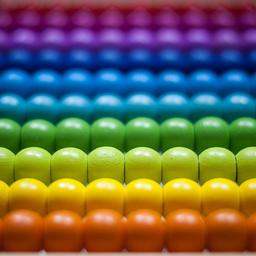
\includegraphics[height=\imgH cm]{Figures/622.jpg}};
\node[above=2pt of imgA, anchor=south, font=\scriptsize] {Edge Map};

\node[imgframe, anchor=west] (imgB) at (0,  -0.5*\inGap)
  {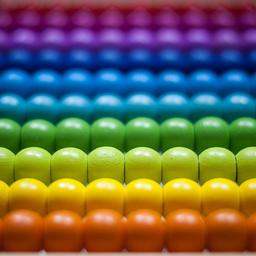
\includegraphics[height=\imgH cm]{Figures/622.jpg}};
\node[below=2pt of imgB, anchor=north, font=\scriptsize] {Image};

% --- Hauptbox-Position: Mittelpunkt zwischen beiden 2cm-Pfeilenden ---
\coordinate (arrowEndA) at ($(imgA.east)+(2cm,0)$);
\coordinate (arrowEndB) at ($(imgB.east)+(2cm,0)$);
\coordinate (boxAnchor)  at ($(arrowEndA)!0.5!(arrowEndB)$);

% --- TSG-Hauptbox ---
\node[bigbox, anchor=west,
      minimum width=\boxW cm, minimum height=\boxH cm] (tsgBox) at (boxAnchor) {};

% Titel oben mittig
\node[font=\bfseries, anchor=north, text=black]
  at ([yshift=-4pt]tsgBox.north) {TSG};

% ================== Innere erste Funktionsbox (DynamicBlur) ==================
\node[fun, anchor=north west] (dynBlur)
  at ([xshift=\padX cm, yshift=-7.5 cm] tsgBox.north west)
  {DynamicBlur};

% Pfeil von Input B (Image) direkt in die Funktionsbox
\draw[flow]
  (imgB.east) -- (dynBlur.west)
  node[flowlabel, above] {Image};

% ------------------ Random Fan-out: genau EINE der drei Varianten ----------------
% Fächerpunkt rechts der Funktionsbox
\coordinate (split) at ($(dynBlur.east)+(\fanout cm,0)$);

% Drei Thumbnails ÜBEREINANDER
\node[imgframe, anchor=west] (thumbGray)
  at ($(split)+(\toThumb cm,  2*\thumbVsep cm)$)
  {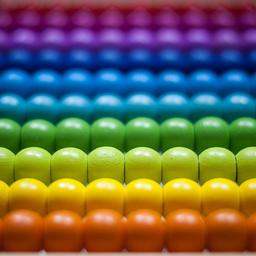
\includegraphics[height=\thumbH cm]{Figures/622.jpg}};
\node[anchor=south] at ([yshift=-2.5pt]thumbGray.north) {All-gray (dropout)};

\node[imgframe, anchor=west] (thumbHeavy)
  at ($(split)+(\toThumb cm,  \thumbVsep cm)$)
  {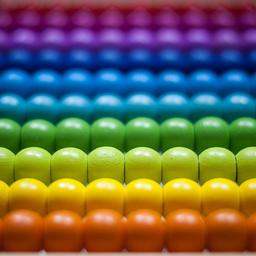
\includegraphics[height=\thumbH cm]{Figures/622.jpg}};
\node[anchor=south] at ([yshift=-2.5pt]thumbHeavy.north) {Heavy blur};

\node[imgframe, anchor=west] (thumbDown)
  at ($(split)+(\toThumb cm, 0cm)$)
  {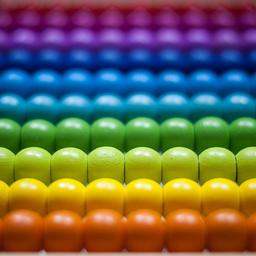
\includegraphics[height=\thumbH cm]{Figures/622.jpg}};
\node[anchor=south] at ([yshift=-2.5pt]thumbDown.north) {Downscale blur};

% Gestrichelte Alternativ-Pfeile direkt vom Filter zu den drei Outputs
\draw[altflow] (dynBlur.east) -- (thumbGray.west)
  node[flowlabel, above] {$p_{\text{zero}}$};
\draw[altflow] (dynBlur.east) -- (thumbHeavy.west)
  node[flowlabel, above] {$p_{\text{heavy}}$};
\draw[altflow] (dynBlur.east) -- (thumbDown.west)
  node[flowlabel, above] {$p_{\text{down}}$};

% Senkrechte Klammer rechts der drei Alternativen
\draw[decorate,decoration={brace, amplitude=4pt}]
  ($(thumbGray.north east)+(10pt,0)$) -- ($(thumbDown.south east)+(10pt,0)$)
  node[flowlabel, xshift=18pt] {random};


% === Ausgangspunkt "rechts der Klammer" und Pfeil zu neuem Bild in TSG ===
% Punkt etwas rechts neben der Klammer (ungefähr mittig der drei Thumbs)
\coordinate (pickOut) at ($(thumbHeavy.east)+(1.6cm,0)$);

% Neues Bild (Generator) innerhalb der TSG-Box, rechts der Thumbs
\node[imgframe, anchor=west, fill=white] (genFig)
  at ([xshift=1.2 cm, yshift=-3.5 cm] tsgBox.north west)
  {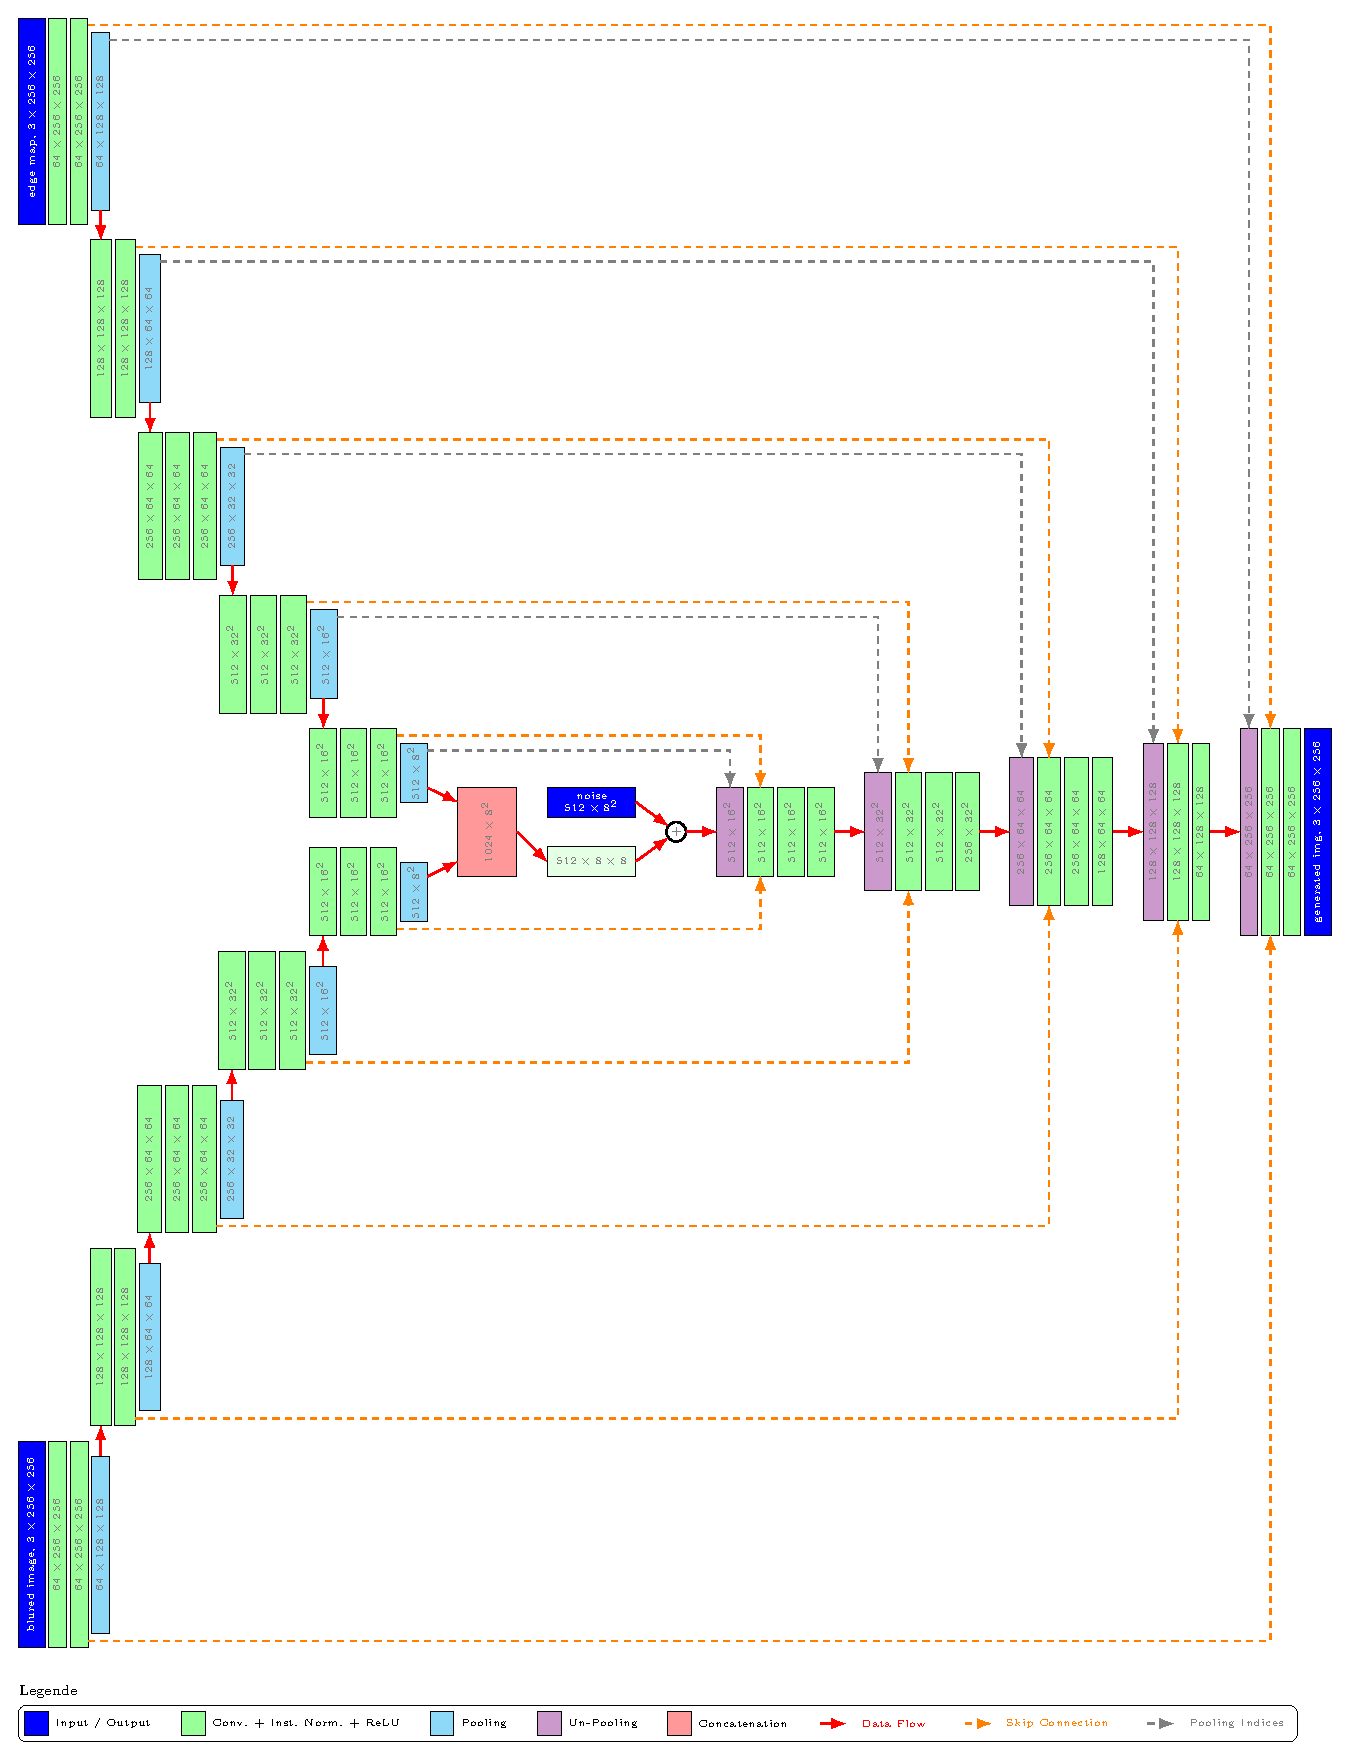
\includegraphics[height=4.3cm]{Figures/Generator_V2_2.pdf}};
\node[above=12pt of genFig, anchor=north, font=\scriptsize] {Encoder-Decoder-Network};

% --- Segmentierter Pfeil: dynBlur.north -> (hoch) -> (links) -> (hoch) -> genFig.south west
\coordinate (k1) at ($(dynBlur.north)+(0,6mm)$);   % etwas nach oben
\coordinate (k2) at ($(k1)+(-1.6cm,0)$);           % dann nach links
\coordinate (k3) at ($(k2)+(0,1.8cm)$);            % wieder nach oben
% Jetzt im rechten Winkel nach rechts genau an die Westkante von genFig:
\draw[flow,shorten >=1pt]
  (dynBlur.north) -- (k1) -- (k2)
  -- node[flowlabel, right, xshift=-8pt, yshift=-7pt] {Texture Map} % mittig auf Segment k2->k3
  (k3) -- (genFig.west |- k3);

\draw[flow]
  (imgA.east) -- ([yshift=1.9cm]genFig.west)
  node[flowlabel, above] {Edge Map};

% --- Rechtes Output-Bild (gleiche Höhe/Größe, Abstand 2 cm) ---
% 1) y-Referenz am Generator (Startpunkt des Pfeils)
\coordinate (genEastShift) at ([yshift=0.12cm]genFig.east);

% 2) Rechtes Bild so platzieren, dass seine Westkante das gleiche y hat
\node[imgframe, anchor=west] (imgR)
  at ($(tsgBox.east |- genEastShift)+(2cm,0)$)
  {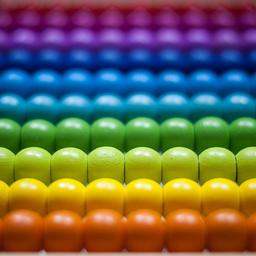
\includegraphics[height=\imgH cm]{Figures/622.jpg}};
\node[above=2pt of imgR, anchor=south, font=\scriptsize] {Generated Image};

% 3) Horizontaler Pfeil (wagrecht), automatisch mittig auf dieser y-Höhe
\draw[flow]
  (genEastShift) -- (imgR.west);

% (Später: Weiterer Flow von der gewählten Variante Richtung imgR)

\end{tikzpicture}
\end{document}
